\chapter{РЕЗУЛЬТАТЫ И ИХ СРАВНИТЕЛЬНЫЙ АНАЛИЗ} \label{ch4}
	Для демонстрации работы предлагаемого решения и сравнения производительности с существующими решениями, в системе визуализации трехмерных сцен \say{DX12Enigne} была реализована поддержка симуляции и визуализации тканей, с возможностью динамического переключения алгоритма симуляции тканей. В качестве эталонного сравнения рассматривается работа библиотеки NVidia Cloth. Для проведения экспериментов были созданы две тестовые сцены, демонстрирующие различые аспекты поведени симулируемой ткани. 
	
	Первая сцена представляет собой открытую городскую местность, в которой размещен флаг, развевающийся на сильном ветру. Движение флага задаётся при помощи системы симуляции тканей. При использовании библиотеки Nvidia Cloth флаг совершает циклические колебания с высокой амплитудой, подобные поведению пружины с грузом под действитем силы тяжести (\firef{fig:flagStreching}). При использовании эвристического алгоритма, описанного в параграфе \ref{ch3:heuristic} подобного поведения не наблюдается (\firef{fig:flagNotStreching}).
	
	\begin{figure}[ht!] 
		\center
		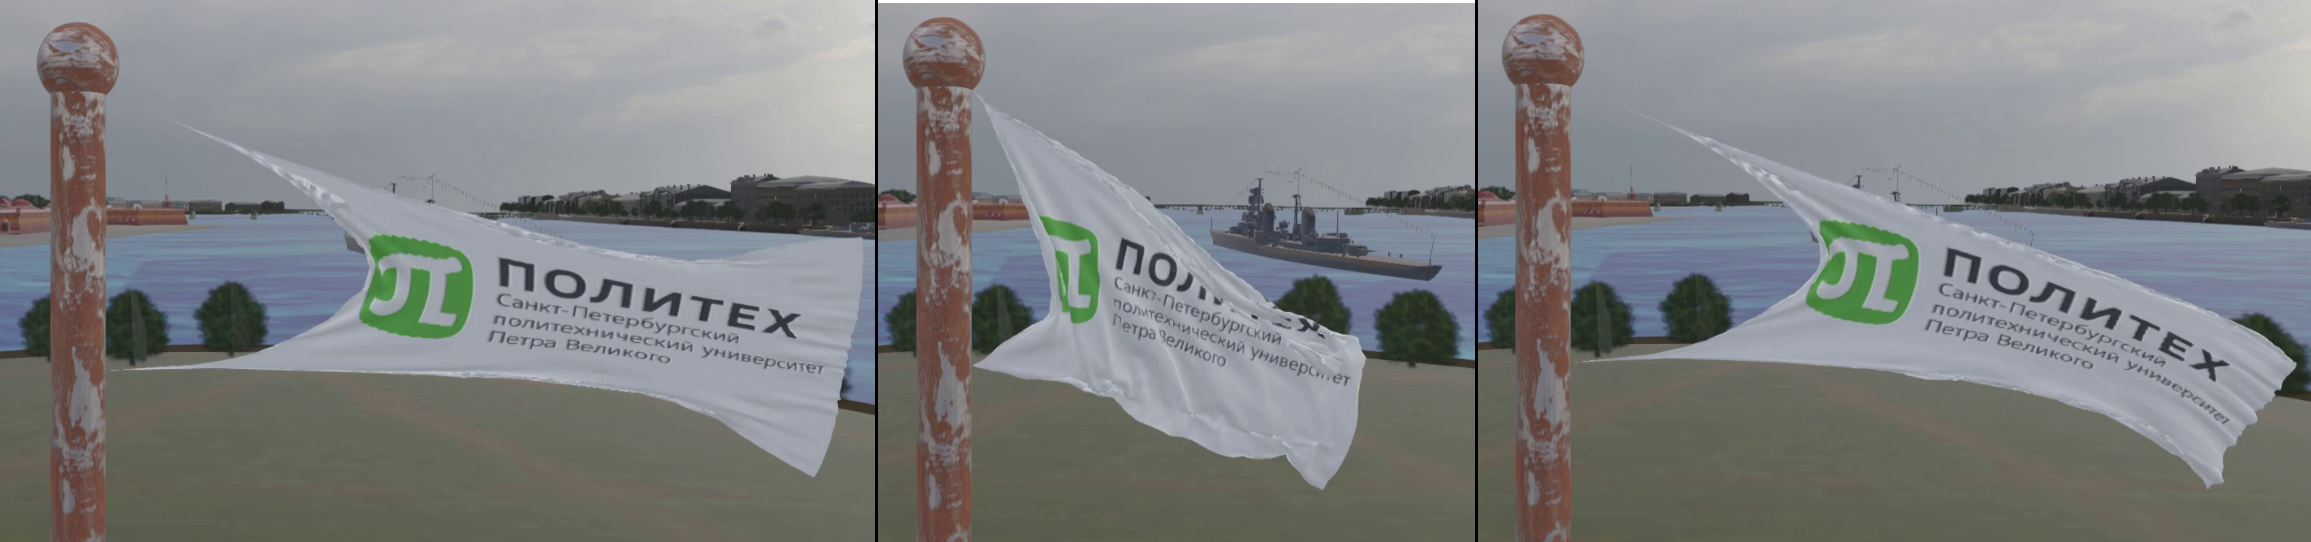
\includegraphics [scale=0.25] {my_folder/images//streching}	
		\caption{Тестова сцена "Флаг". Используется Nvidia Cloth. Кадры спустя 1, 2 и 3 секунды после запуска симуляции.} 
		\label{fig:flagStreching}
	\end{figure}
	
	\begin{figure}[ht!] 
		\center
		
\includegraphics [scale=0.2] {my_folder/images//notStreching}	
		\caption{Тестова сцена "Флаг". Используется эвристический алгоритм. Кадры спустя 1, 2 и 3 секунды после запуска симуляции.} 
		\label{fig:flagNotStreching}
	\end{figure}
	
	\FloatBarrier
	
	Вторая сцена представляет собой учебную аудиторию, в которой находится танцующая девушка. Из окна падает свет солнца, оставляя в помещении динамические тени. Девушка при этом одета в юбку, которая в свою очередь симулируется как поверхность ткани, состоящая из 2048 частиц, 2016 структурных ограничений и 2016 ограничений сдвига. Дополнительно обрабатываются пересечения с ногами и торсом девушки за счет упрощенного представления их как капсул. Также используется алгоритм устранения самопересечений из параграфа \ref{ch3:selfCollision}. Алгоритм симуляции использует технику Small steps, разделяя шаг на 30 подшагов. Примеры кадров представлены на \firef{fig:dance1}, \firef{fig:dance2}, \firef{fig:dance3}.
	
	\begin{figure}[ht!] 
		\center
		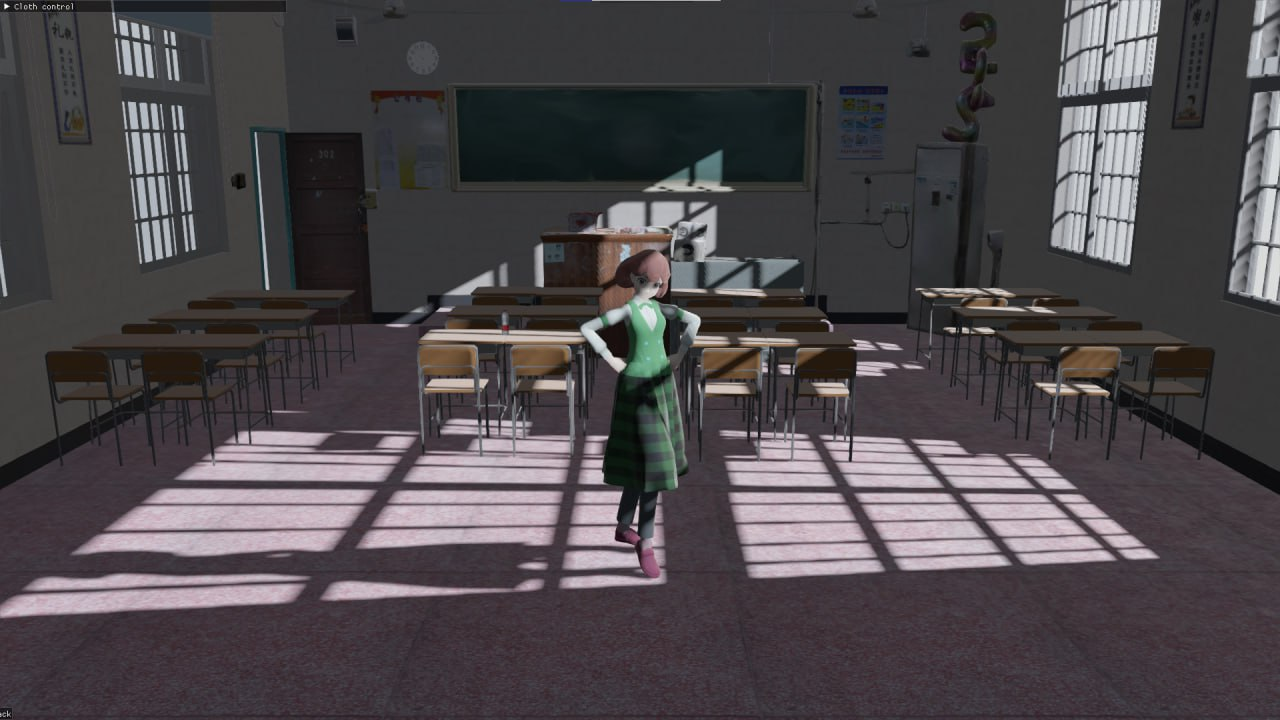
\includegraphics [scale=0.35] {my_folder/images//dance1}	
		\caption{Тестовая сцена "Танец". Кадр записанный в начале анимации} 
		\label{fig:dance1}
	\end{figure}

	\begin{figure}[ht!] 
		\center
		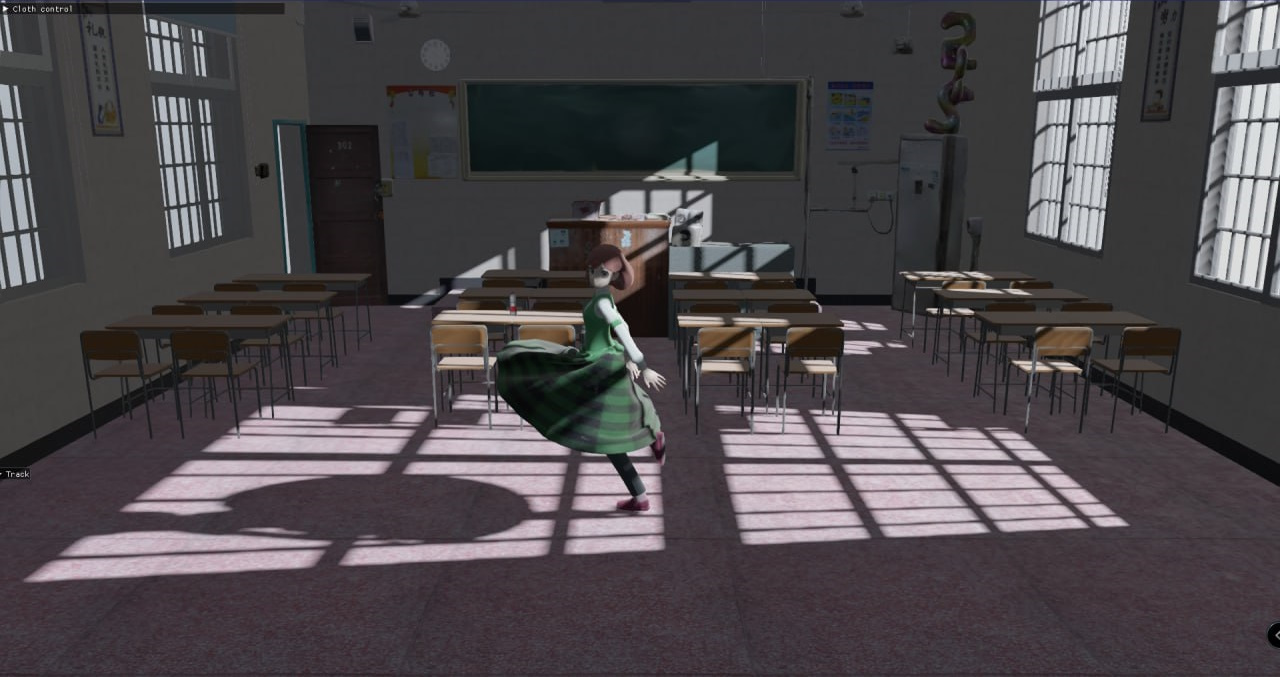
\includegraphics [scale=0.35] {my_folder/images//dance2}	
		\caption{Тестовая сцена "Танец". Кадр записанный в середине анимации} 
		\label{fig:dance2}
	\end{figure}

	\begin{figure}[ht!] 
		\center
		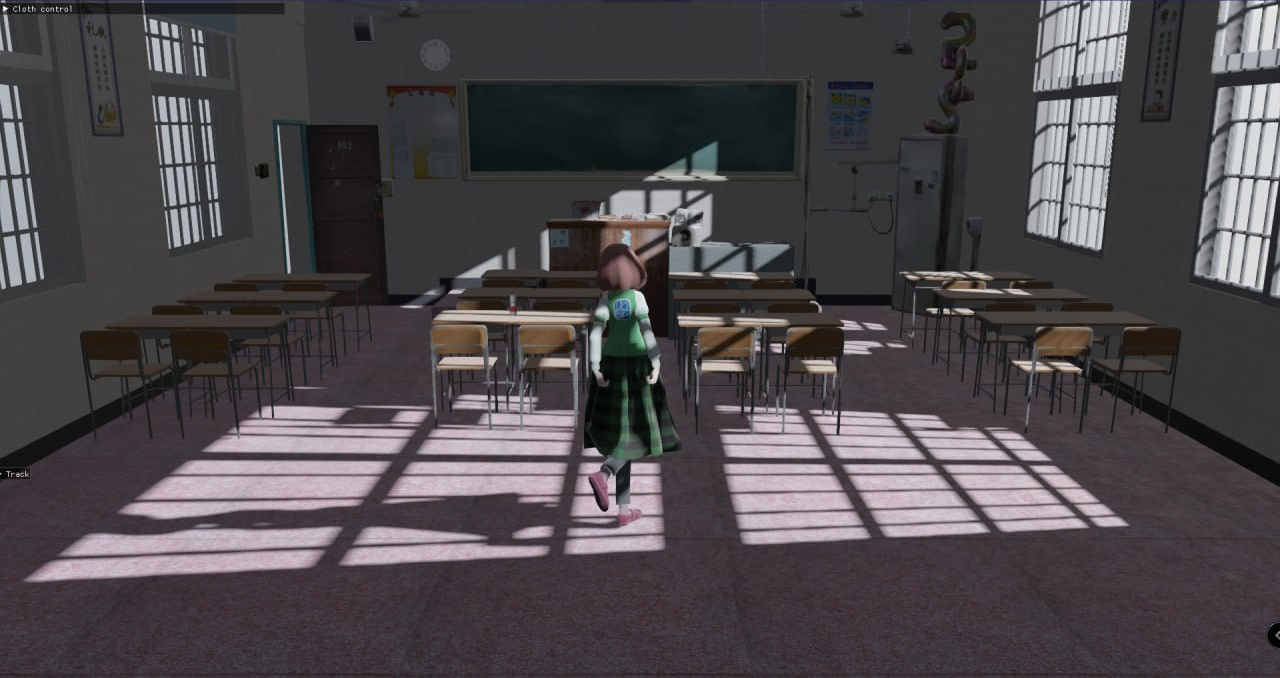
\includegraphics [scale=0.35] {my_folder/images//dance3}	
		\caption{Тестовая сцена "Танец". Кадр записанный в конце анимации} 
		\label{fig:dance3}
	\end{figure}
	
	\FloatBarrier
	
	На данной сцене производилось измерение длительности работы алгоритма симуляции тканей в течение всей анимации, для разных алгоритмов симуляции. Результаты представлены на графике (\firef{fig:solversPlot}). Значения \say{Nvidia Cloth} соответствуют времени работы реализации, используемой в библиотеке Nvidia Cloth на GPU, а значения \say{Me} соответствуют времени работы разработанной автором реализации алгоритма XPBD с применением всех описанных оптимизаций. Эксперименты проводились на компьютере, характеристики которого представленны в таблице \ref{tab:spec}.
	
	\begin{table}[ht]
		\caption{Характеристики компьютера, на котором проводилось тестирование}
		\label{tab:spec}
		\centering
		\begin{SingleSpace}
			\begin{tabular}{|c|c|}
				\hline
				CPU & Intel Core 
				i5-9600K
				\\
				\hline
				GPU & nVidia RTX 2070 SUPER \\
				\hline
				RAM & 32 Gb \\
				\hline
		\end{tabular}
		\end{SingleSpace}
	\end{table}
	
	\begin{figure}[ht!] 
		\center
		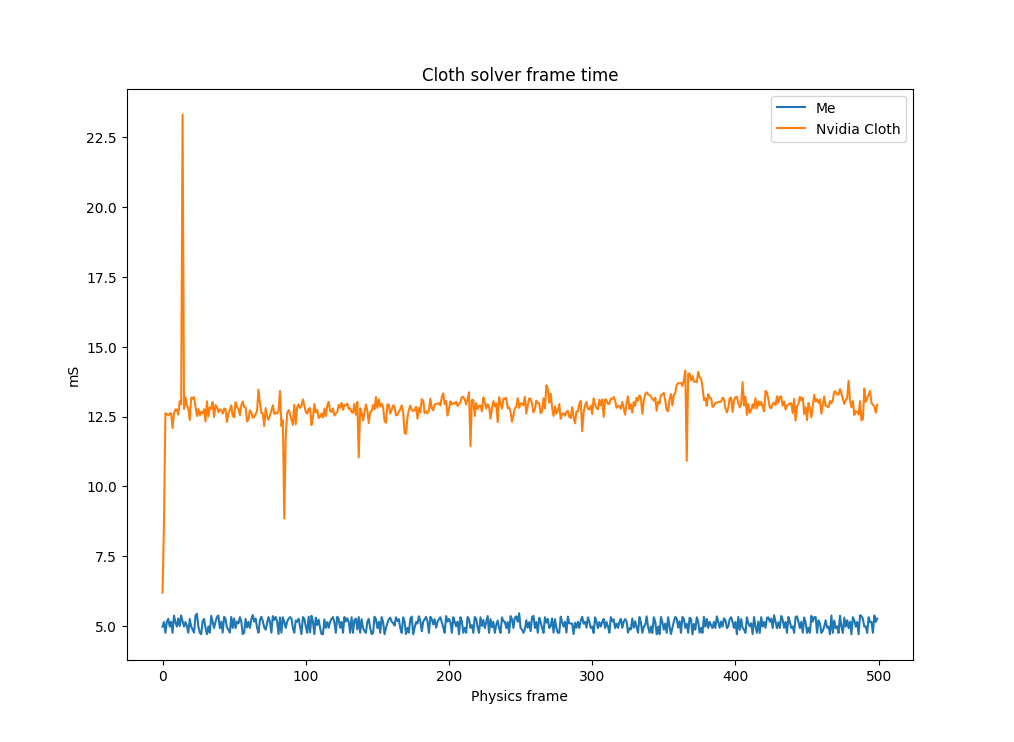
\includegraphics [scale=0.7] {my_folder/images//frameTimePlot}	
		\caption{График времени работы алгоритма симуляции тканей. По оси X отложен номер кадра анимации, по оси Y - время работы системы симуляции в миллисекундах. Среднее время работы Nvidia Cloth равно 12.87ms, среднее время работы предлагаемого алгоритма - 5.06ms. } 
		\label{fig:solversPlot}
	\end{figure}
	\FloatBarrier
	
	Исходя из кадров, представленных на \firef{fig:flagStreching} и \firef{fig:flagNotStreching}, можно заметить, что предлагаемый эвристический алгоритм позволяет бороться с циклическими колебаниями, связанными с влиянием больших по модулю сил. При этом, исходя из \firef{fig:solversPlot}, можно заметить, что использование всех предлагаемых оптимизаций позволяет производить симуляции более чем в два раза быстрее, чем это может быть сделано с использованием библиотеки Nvidia Cloth, признанной стандартом индустрии.
	
%Хорошим стилем является наличие введения к главе. Во введении может быть описана цель написания главы, а также приведена краткая структура главы. 
	
%\section{Название параграфа} \label{ch4:sec1}

%\section{Название параграфа} \label{ch4:sec2}

%Пример ссылки на литературу \cite{avtonomova:fya,Peskov2004-ru,Kotelnikov2004-ru,Kotelnikov2004}.

%\FloatBarrier % заставить рисунки и другие подвижные (float) элементы остановиться

%\section{Выводы} \label{ch4:conclusion}

%Текст выводов по главе \thechapter.

%% Вспомогательные команды - Additional commands
%
%\newpage % принудительное начало с новой страницы, использовать только в конце раздела
%\clearpage % осуществляется пакетом <<placeins>> в пределах секций
%\newpage\leavevmode\thispagestyle{empty}\newpage % 100 % начало новой страницы